\vspace{-2em}
\section{Αποτελέσματα}
\label{Final_Results}

Στα τρία προηγούμενα κεφάλαια παρουσιάστηκε η διαδικασία εκπαίδευσης δύο νευρωνικών δικτύων ικανών να διακρίνουν και να ταξινομήσουν διαφορετικά είδη τροφών με τη χρήση εικόνων. Όπως αναφέρθηκε τα μοντέλα που επιλέξαμε ήταν το ResNet50mod (1) και το ResNet50mod\_transfer (3). 

Στον παρακάτω πίνακα \ref{final_results_table}
φαίνονται τα αποτελέσματα για την ακρίβεια, λεπτομέρεια (precision), ευαισθησία (recall) και την ακρίβεια top-5 για τα δύο μοντέλα. Επιπλέον στον ίδιο πίνακα αναγράφεται και η ακρίβεια αναφοράς (baseline accuracy) , η οποία ορίζεται ως η ακρίβεια που θα επιτύγχανε ένας αλγόριθμος που θα απέδιδε σε όλες τις παρατηρήσεις την πιο συχνά εμφανιζόμενη κατά την εκπαίδευση κλάση.  Σαν δεδομένα ελέγχου χρησιμοποιήθηκαν αυτά του test συνόλου δεδομένων που δεν είχαν χρησιμοποιηθεί μέχρι αυτό το τελικό στάδιο. Οι τρεις πρώτοι δείκτες υπολογίζονται από τις σχέσεις \ref{eval_relations}.  

Πρέπει να σημειωθεί ότι ενώ η ακρίβεια μπορεί να υπολογιστεί απευθείας διαιρώντας τις σωστές προβλέψεις με το σύνολο των προς πρόβλεψη σημείων, ο υπολογισμός για τους άλλους δύο δείκτες δεν είναι τόσο απλός. Αυτό γιατί πρέπει να υπολογιστεί η λεπτομέρεια (ή ισοδύναμα η ευαισθησία) για κάθε κλάση και στη συνέχεια παίρνοντας τον σταθμισμένο μέσο όρο να υπολογιστεί για το σύνολο του προβλήματος. 

Αναφορικά με τον ορισμό της ακρίβειας top-5, χρησιμοποιείται το ακόλουθο. Ο αλγόριθμος πρόβλεψης επιστρέφει τις πιθανότητες η κάθε εικόνα του test να ανήκει σε κάποια από τις 256 για το πρώτο ή 101 για το δεύτερο πρόβλημα κλάσεις. Έτσι αν η σωστή απάντηση βρίσκεται σε κάποια από τις πέντε επικρατέστερες κλάσεις τότε η απάντηση θεωρείται σωστή. 

Κλείνοντας στο σχήμα δίνεται ο πίνακας σύγχυσης (confusion matrix) \ref{confusion_matrix_fig_1} για το πρώτο πρόβλημα και αντίστοιχα στο σχήμα \ref{confusion_matrix_fig_2} για το δεύτερο πρόβλημα.

\begin{subequations} \label{eval_relations}
\begin{gather}
ACC=\dfrac{TP+TN}{P+N} \label{accuracy} \tag{4.1.1a}\\
PPV_{class}=\dfrac{TP}{TP+FP} \label{precision_PPV} \tag{4.1.1b}\\
SEN_{class}=\dfrac{TP}{TP+FN} \label{recall} \tag{4.1.1c}\\
\begin{cases}
\begin{aligned}
TP : True \, Positive, \, FP : False \, Positive \\
TN : True \, Negative, \, FN : False \, Negative 
\end{aligned} \tag{4.1.1e}
\end{cases}
\end{gather}
\end{subequations}


\begin{table}[H]
\centering
\begin{tabular}{|cc|cc|}
\hline
\multicolumn{2}{|c|}{UECFOOD256}         & \multicolumn{2}{c|}{FOOD101}            \\ \hline
\multicolumn{1}{|c|}{Baseline Accuracy}  & 0.02186 & \multicolumn{1}{c|}{Baseline Accuracy}       & 0.01386 \\ \hline
\multicolumn{1}{|c|}{Accuracy}       & 0.76751 & \multicolumn{1}{c|}{Accuracy}       & 0.63415 \\ \hline
\multicolumn{1}{|c|}{Top-5 Accuracy} & 0.90764 & \multicolumn{1}{c|}{Top-5 Accuracy} & 0.82607 \\ \hline
\multicolumn{1}{|c|}{Precision}      & 0.78941 & \multicolumn{1}{c|}{Precision}      & 0.64691 \\ \hline
\multicolumn{1}{|c|}{Recall}         & 0.76751 & \multicolumn{1}{c|}{Recall}         & 0.63534 \\ \hline
\end{tabular}
\caption{Τελικά αποτελέσματα}
\label{final_results_table}
\end{table}


\begin{figure}[H]
\centering
\begin{subfigure}[t]{1.0\textwidth}%
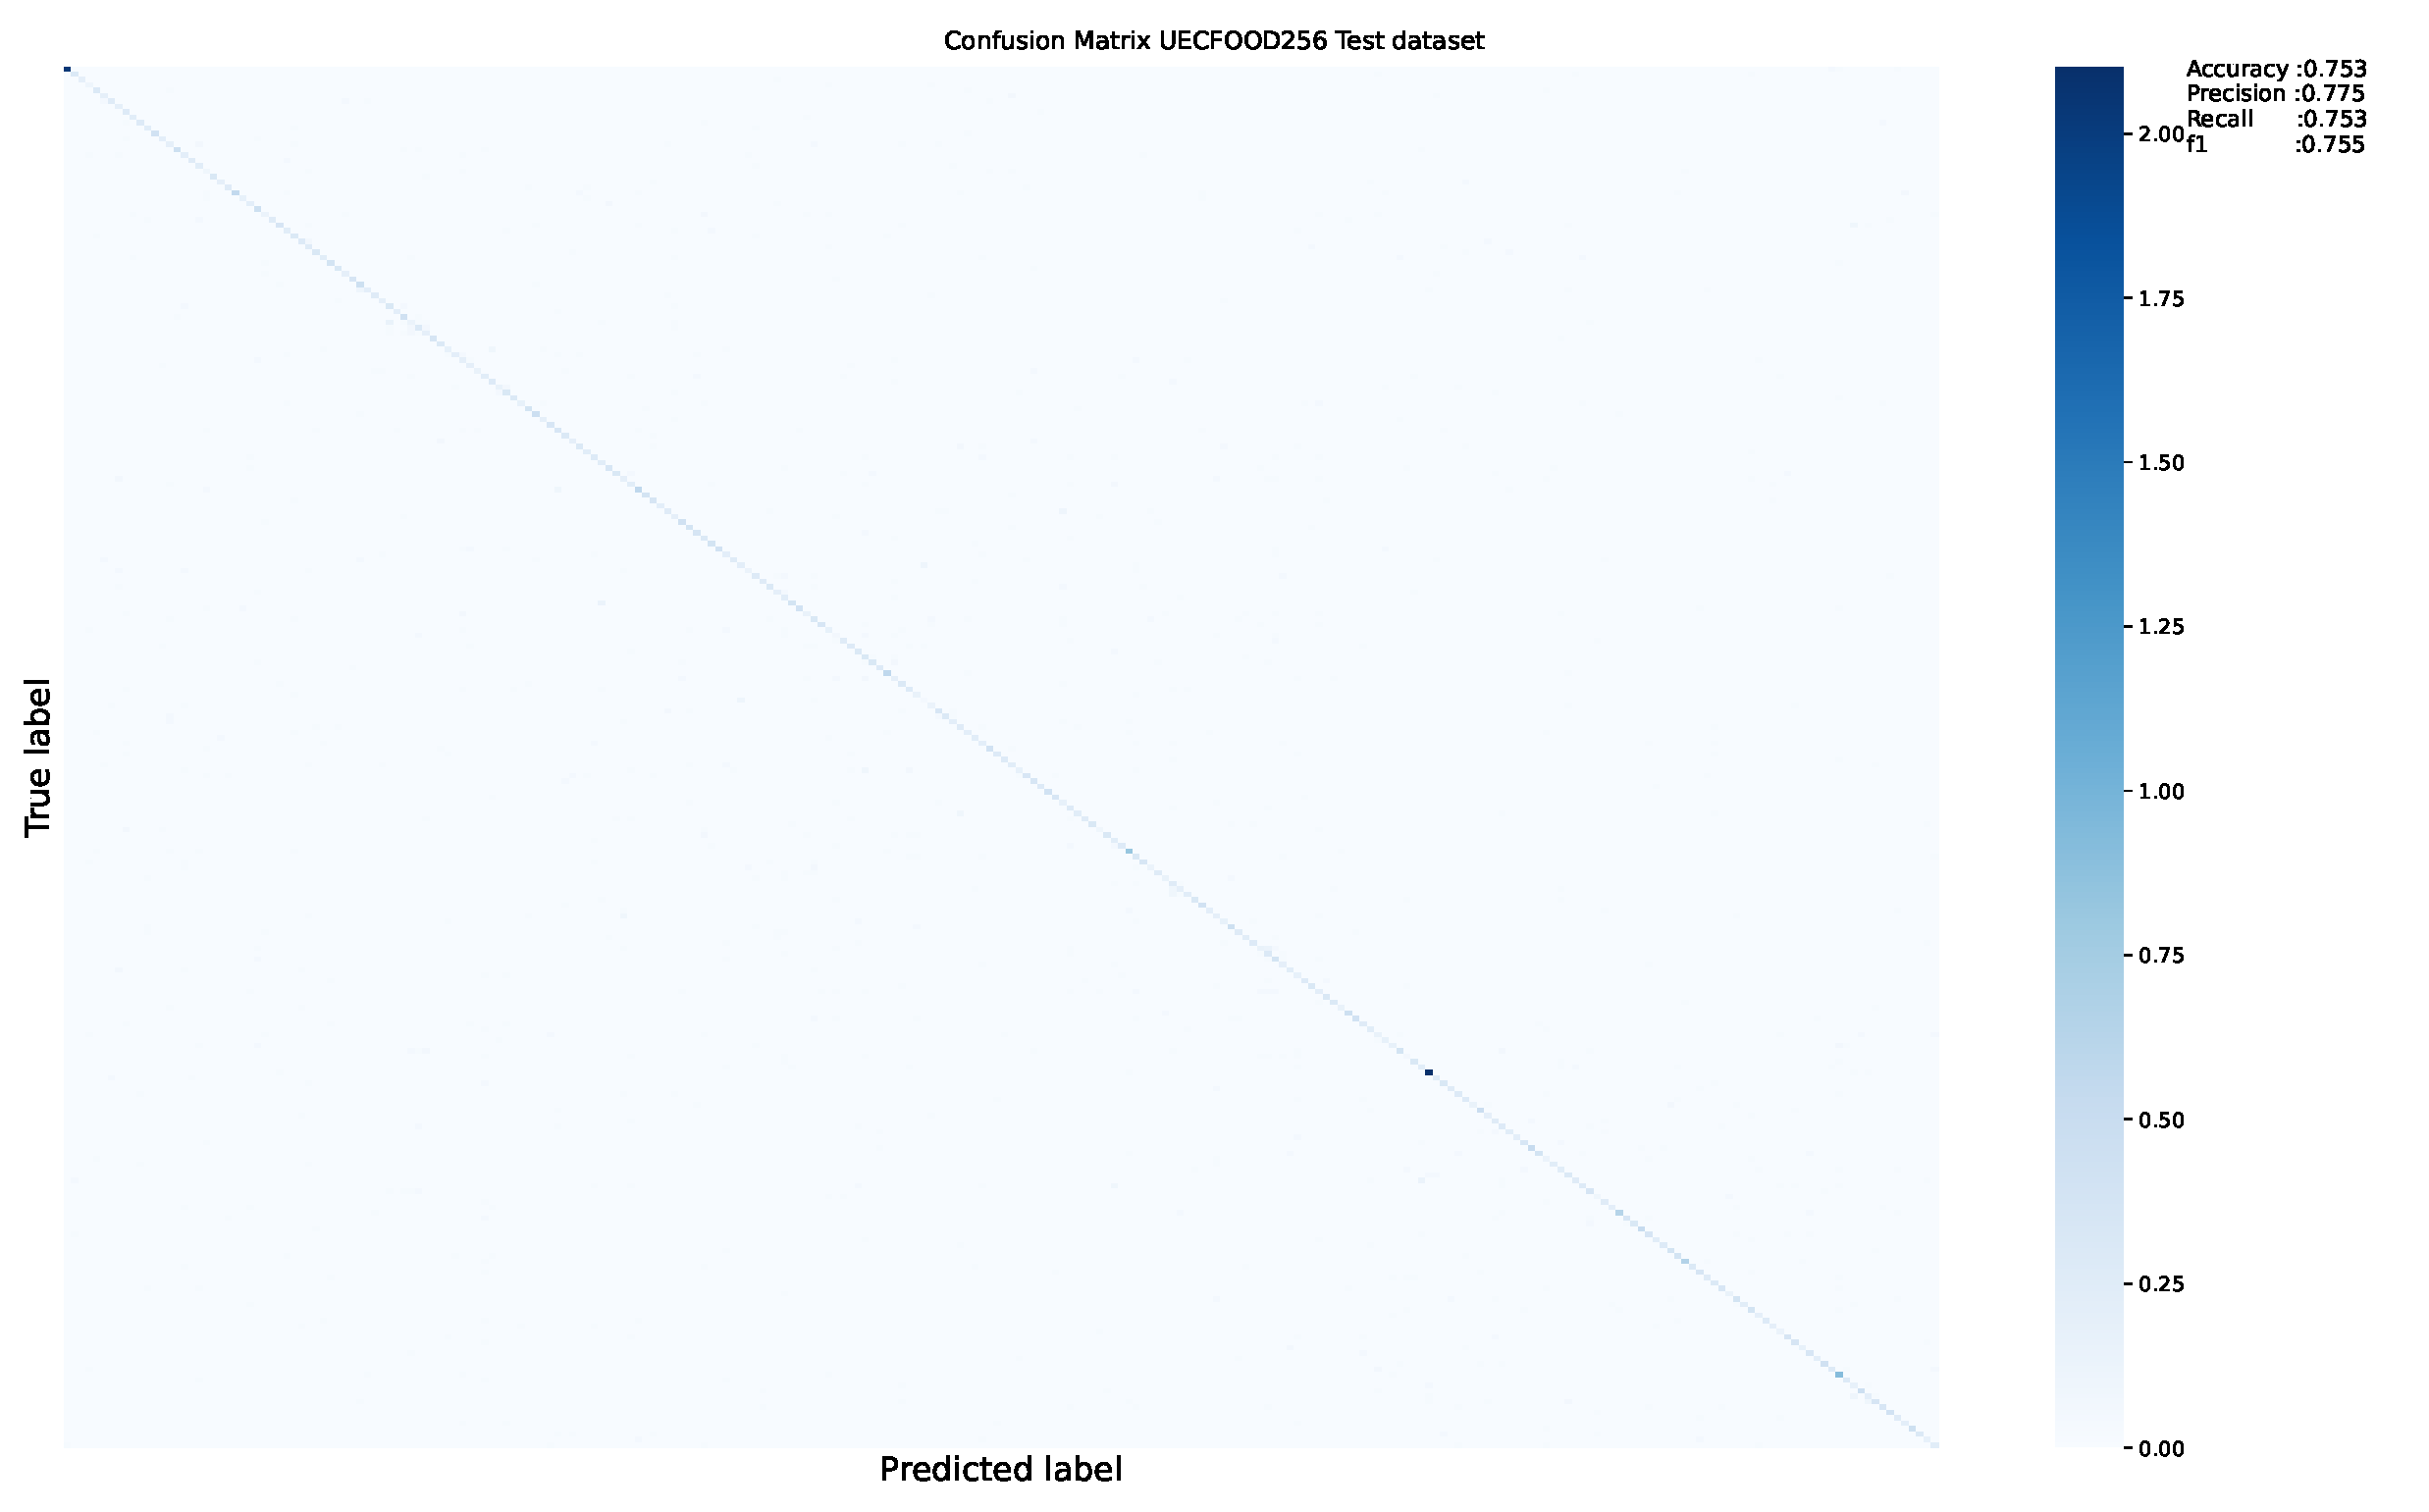
\includegraphics[width=\textwidth]{conf_matrix_dataset_1_(256, 256)_ResNet50mod_generator_2_regularizer_no_nlu1_20.pdf}
\end{subfigure}
\caption{Confusion matrix ResNet50mod}
\label{confusion_matrix_fig_1}
\end{figure}


\begin{figure}[H]
\centering
\begin{subfigure}[t]{1.0\textwidth}%
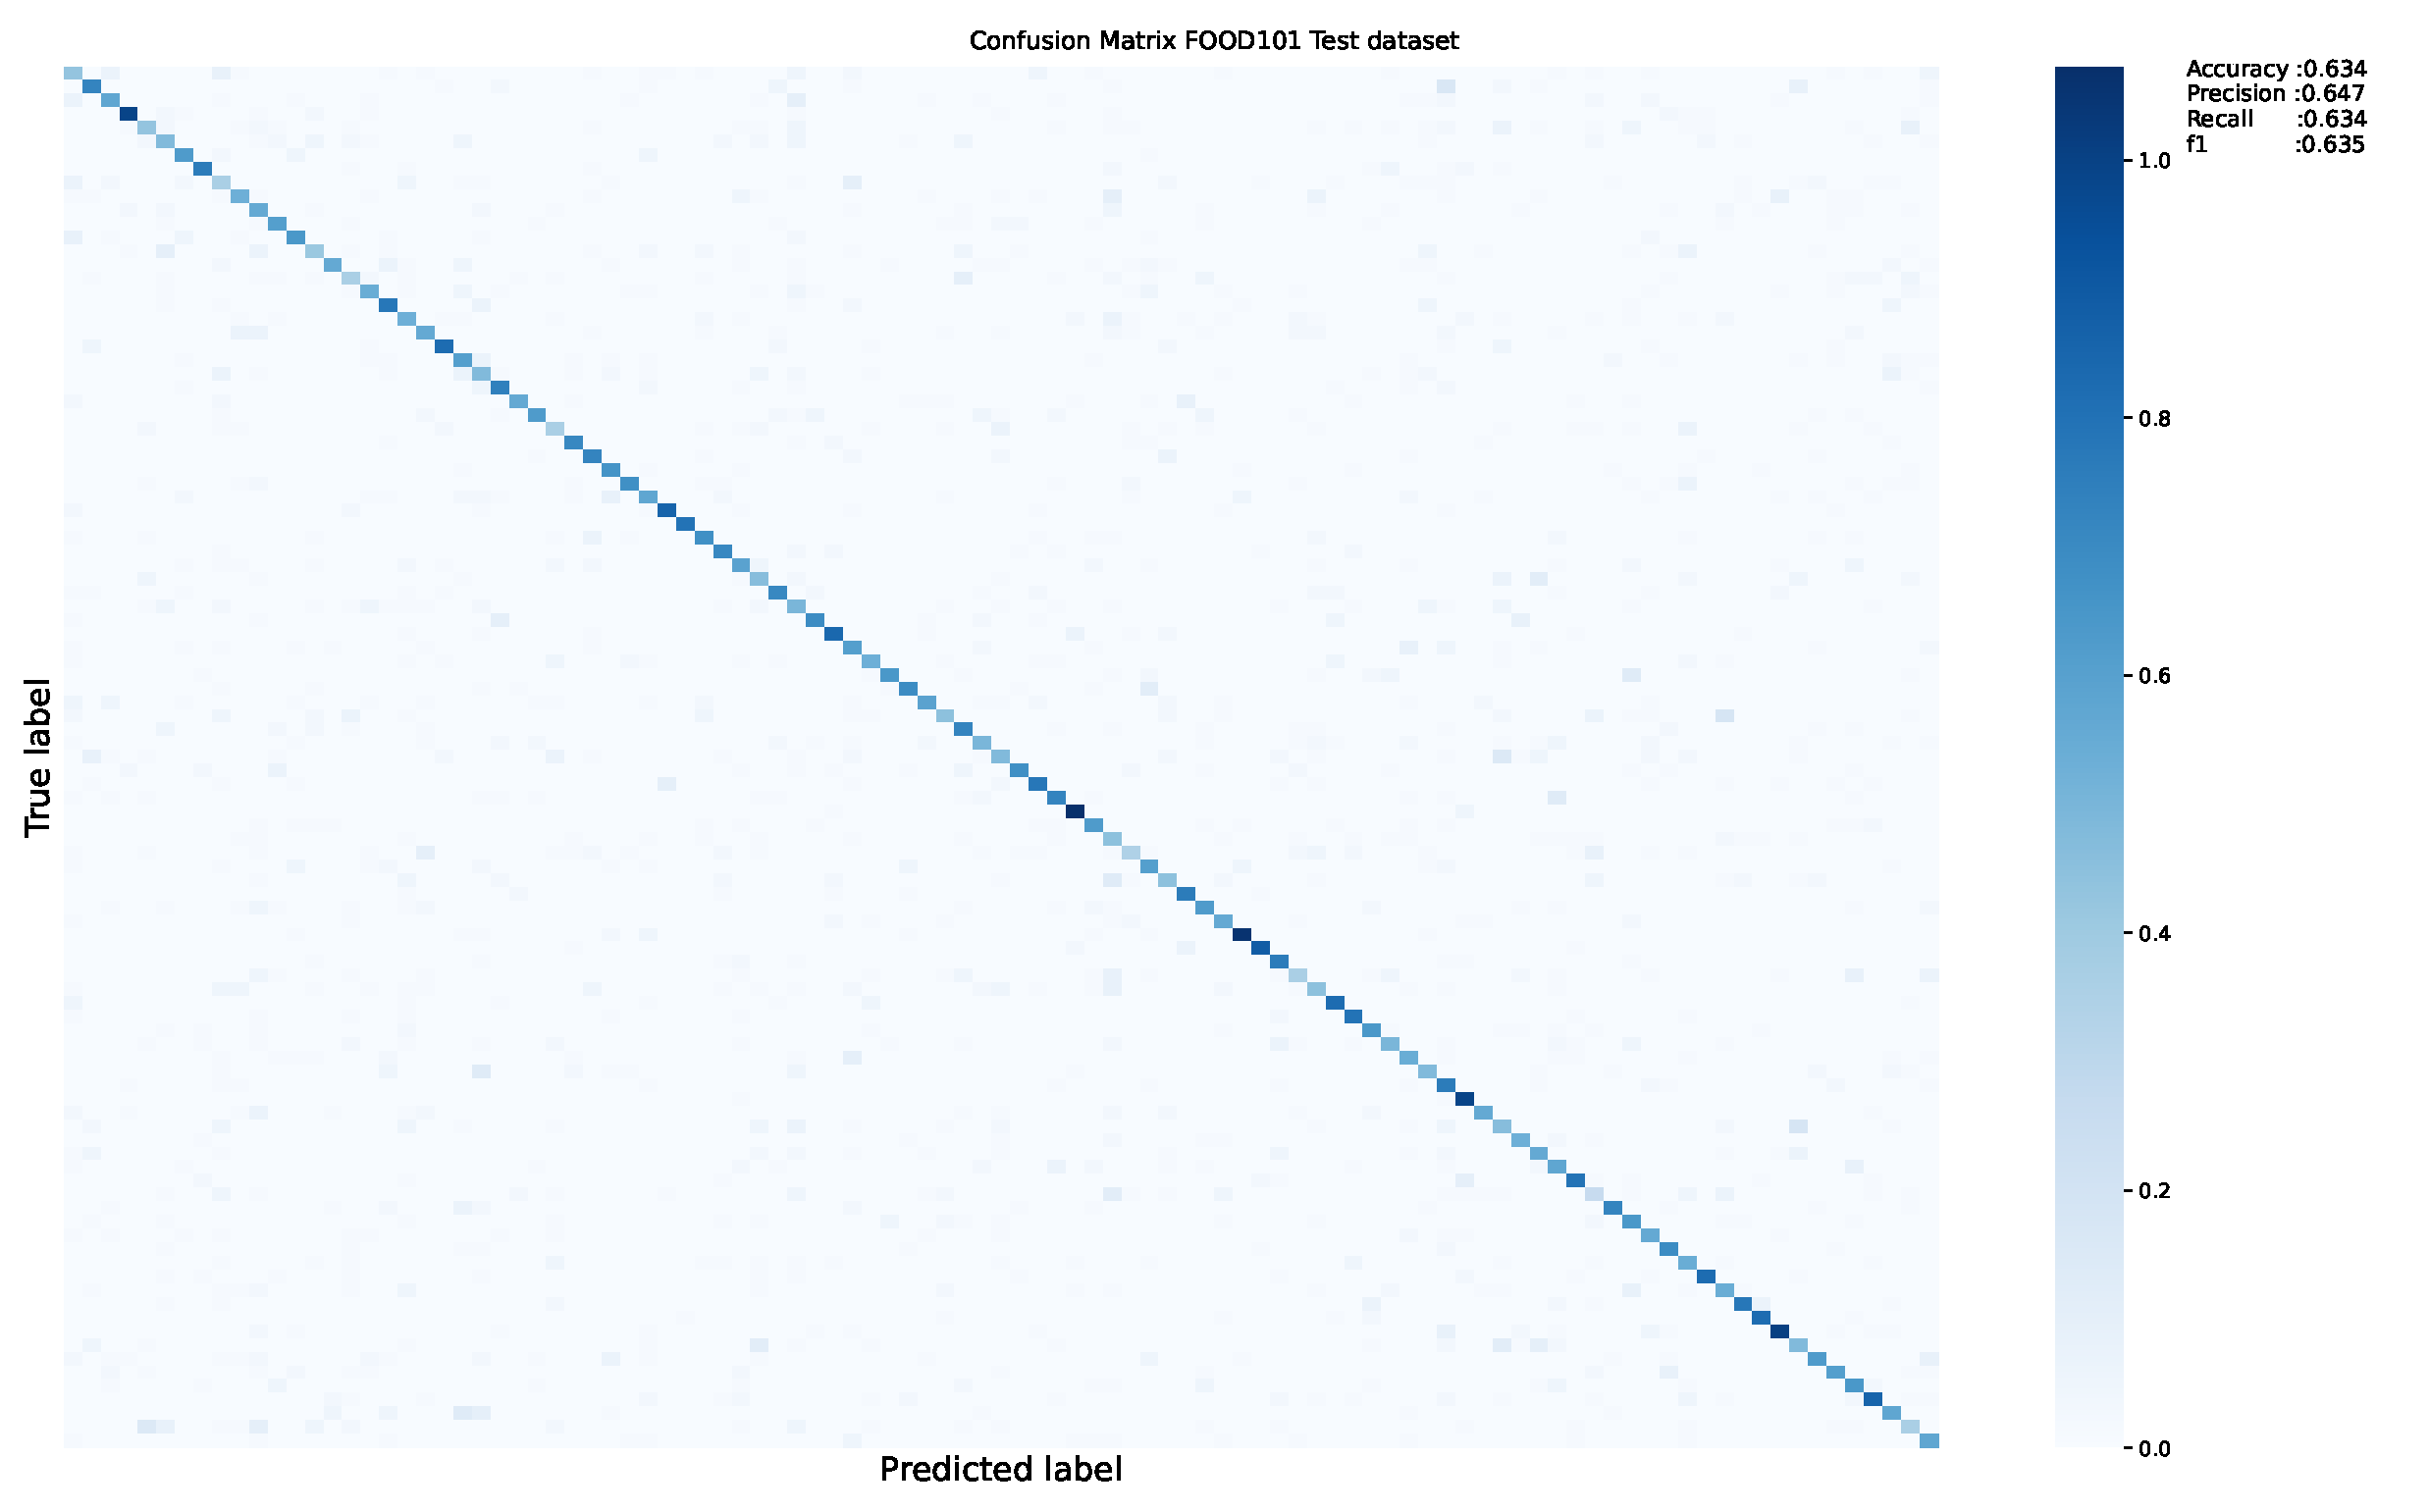
\includegraphics[width=\textwidth]{conf_matrix_dataset_2_(256, 256)_ResNet50mod_generator_2_regularizer_no_nlu1_20_nlu2_14.pdf}
\end{subfigure}
\caption{Confusion matrix ResNet50mod\_transfer}
\label{confusion_matrix_fig_2}
\end{figure}



\section{Συμπεράσματα}
\label{Conclusions}

Οι προκλήσεις που αντιμετωπίστηκαν κατά τη διάρκεια της εκπαίδευσης οφείλονταν σε μια σειρά παραμέτρων και περιγράφηκαν σε διάφορα σημεία της αναφοράς. Συνοπτικά μπορούν να κατηγοριοποιηθούν στις παρακάτω κατηγορίες.

\begin{enumerate}
\item Επάρκεια υπολογιστικών πόρων (μνήμης RAM) και χρόνου εκτέλεσης
\item Πλήθος υπερπαραμέτρων και εντοπισμός βέλτιστης λύσης 
\item Προλήματα overfitting και underfitting
\end{enumerate}


Αναλυτικότερα, η επάρκεια υπολογιστικών πόρων είναι σημαντική για όλα τα προβλήματα deep learning καθώς ο όγκος των δεδομένων είναι ιδιαίτερα μεγάλος με αποτέλεσμα ένας απλός οικιακός υπολογιστής να μην μπορεί να ανταπεξέλθει. Το πρόβλημα δεν αφορά μόνο την ταχύτητα επεξεργασίας των δεδομένων, αλλά επίσης και τις απαιτήσεις σε μνήμη RAM. Για τον λόγο αυτό, στην παρούσα εργασία ήταν αδύνατον να χρησιμοποιηθεί κάποιο υπάρχον διαδικτυακό μέσον που εκτελεί τον κώδικα παράλληλα, καθώς η RAM ξεπερνούσε τα 25-30 GB με αποτέλεσμα να μην μπορεί να εκτελεστεί. Έτσι καταφύγαμε στη λύση του οικιακού υπολογιστή με αποτέλεσμα να μην παραλληλοποιηθεί η διαδικασία μας.

Το πλήθος των υπερπαραμέτρων προς προσδιορισμό (tuning) είναι πολύ μεγάλο και όπως είδαμε λόγω και του αυξημένου χρόνου είναι αδύνατο να κάνουμε ακριβή προσδιορισμό του βέλτιστου συνδυασμού. Κατά συνέπεια, μελετήθηκαν κάποιες  ενδεικτικές περιπτώσεις, οπότε είναι πιθανό ότι μια πιο ενδελεχής δοκιμή υπερπαραμέτρων θα οδηγούσε σε ακόμη καλύτερα αποτελέσματα.

Τα προβλήματα overfitting και underfitting ήταν παρόντα σε διάφορες περιπτώσεις. Έτσι όταν δεν είχαμε πολλά layers προς εκπαίδευση δεν πετυχαίναμε επαρκή ακρίβεια, ενώ αντίθετα όσο αυξάναμε τα layers αύξανε η ακρίβεια αλλά υπήρχε overfitting. Για αυτό το λόγο, χρησιμοποιήσαμε dropout layers το οποίο φάνηκε να βοηθάει τα τελικά αποτελέσματα. Εκ νέου όμως το υπολογιστικό κόστος ήταν απαγορευτικό για μια βαθύτερη μελέτη.
